\documentclass{lgtdslides}

\usepackage{tikz}
\usepackage{tikzsymbols}
\usepackage[american]{babel}

\usepackage{lgtdfigs}

\title{Playing with the lights}
\subtitle{\textit{Control WiFi-enabled LIFX light bulbs}}
\date{Fosdem 2017, IoT track}
\author{Louis Opter <louis@opter.org>}

\tikzset{bubble/.style={fill,opacity=0.7,rounded corners=2pt}}
\tikzset{arrow/.style={->, >=stealth,ultra thick,rounded corners}}
\tikzset{controlpt/.style={opacity=0}}
\tikzset{hidden/.style={opacity=0}}
\tikzset{wifipath/.style={thick,opacity=0.8,decorate,decoration={name=expanding waves,angle=25,segment length=3.5}}}
\tikzset{box/.style={draw,ultra thick, color=BeamerBlue, text=black, rectangle, rounded corners=1pt}}

\begin{document}

\begin{frame}\titlepage\end{frame}

\section{Intro}

\subsection{About me}

\begin{frame}{\LARGE{\texttt{\$ whoami}}}
Hello, my name is Louis (Opter) and I:\vspace{1em}
\begin{itemize}
\item am a decent software engineer;
\item \emph{do not really know anything about hardware.}
\end{itemize}
\vspace{1em}
Anyway, it doesn't really matter, let's get started!
\end{frame}

\subsection{Plan}

\begin{frame}{Agenda}
Two related projects to talk about:
\vspace{1em}
\begin{description}
\item[monolight] An UI for a 128 buttons matrix and lightsd;
\item[lightsd] A daemon to easily control LIFX light bulbs.
\end{description}
\pause
\vspace{2em}
Outline:
\vspace{1em}
\begin{itemize}
\item monolight: explanation, demo, implementation, ideas;
\item lightsd: API demo, implementation, ideas, about LIFX;
\item Q\&A, discussion.
\end{itemize}
\end{frame}

\begin{frame}{High-level architecture}
\begin{center}
\begin{tikzpicture}[overlay]
\coordinate (Origin) at (0,0);

\fill[controlpt] (Origin) circle (0.1);

\node[box] (monolight) at (3.5,0.75) {monolight};
\node[box] (lightsd) at (0.5,-2) {lightsd};
\draw[ultra thick] (-1.46, 1.5) -| (monolight);
\node (monome) at (-3.5,1.5) {\begin{tikzpicture}
\pic (0, 0) {monome={scale 0.5}};
\end{tikzpicture}};
\node (bulbh) at (-4.2,-1.1) {\begin{tikzpicture}
\pic (0, 0) {lightbulb={LightSlateBlue scale 0.19 rotate 90}};
\end{tikzpicture}};
\node (bulbl) at (-4.2,-2.9) {\begin{tikzpicture}
\pic (0, 0) {lightbulb={IndianRed scale 0.19 rotate 90}};
\end{tikzpicture}};

\draw[ultra thick] (lightsd) -| (monolight);
\draw[wifipath] (bulbh.east) -- (-2.2,-1.15);
\draw[wifipath] (lightsd.west) -- (-1.1,-2);
\draw[wifipath] (bulbl.east) -- (-2.2,-2.85);
\onslide<2->{%
\draw[ultra thick,dashed] (-6,-0.2) -- (6,-0.2);
\draw (0,-0.2) node[above] {\emph{Talk part 1 (monolight)}}
               node[below] {\emph{part 2 (lightsd)}};
\fill[white,opacity=0.7] (-6,-6) rectangle (6,-0.2);
}
\end{tikzpicture}
\end{center}
\end{frame}

\section{monolight}

\subsection{Controller UI}

\begin{frame}{monolight}
A controller (Monome grid 128 varibright):
\begin{itemize}
\item A matrix of 128 programmable button;
\item 16 levels of brightness per button;
\item Serial/RS232 (FTDI) connection.
\end{itemize}
\pause
\vspace{1em}
Controlling a "smart" bulb (LIFX Original 1000):
\begin{itemize}
\item A \textasciitilde1000 lumens programmable light bulb;
\item Nice colors, nice range of whites;
\item Wi-Fi 802.11bgn, 2.4gHz.
\end{itemize}
\pause
\vspace{1em}
\emph{Let's have a look at the controller UI.}
\end{frame}

\begin{frame}{The grid}
\begin{center}
\begin{tikzpicture}[overlay]
\pic (0, 0) {monome={scale 1.2}};
\end{tikzpicture}
\end{center}
\end{frame}

\begin{frame}{General functions/scenes row}
\begin{center}
\begin{tikzpicture}[overlay,scale=1.2]
\onslide<1->{%
\pic (0, 0) {monome={scale 1.2}};

\foreach \x in {-4,-3.5,...,3.5}
\fill[mbutton] (\x, -1.75) rectangle +(0.36, -0.36);
}
\onslide<2->{%
\foreach \x in {-1.5,-1,...,3}
\fill[mbuttoff] (\x, -1.75) rectangle +(0.36, -0.36);

\fill[color=fgcolor,decoration={name=snake,amplitude=2,segment length=45}]
  decorate {(-4.25,-1.35) -- (4.15,-1.35)} -- (4.15,2) -- (-4.25,2) -- cycle;

\node[rectangle] (b112) at (-3.82,-1.93) {};
\node[rectangle] (b113) at (-3.32,-1.93) {};
\node[rectangle] (b114) at (-2.82,-1.93) {};
\node[rectangle] (b115) at (-2.32,-1.93) {};
\node[rectangle] (b116) at (-1.82,-1.93) {};
\node[rectangle] (b117) at (-1.32,-1.93) {};
\node[rectangle] (b127) at (3.68,-1.93)  {};
}
\onslide<2>{
\node (toggle) [above=1.1cm of b112] {%
\begin{minipage}{2cm}
\begin{center}
on/off

toggle
\end{center}
\end{minipage}};
\node (off) [above=0.7cm of b113] {off};
\node (on) [above=1.1cm of b114] {on};
\node (scenes) [above=0.7cm of b116] {scenes\ldots};
\node (uitoggle) [above=1.1cm of b127] {toggle UI};

\draw[arrow] (toggle) -- (b112);
\draw[arrow] (off) -- (b113);
\draw[arrow] (on) -- (b114);
\draw[arrow] (uitoggle) -- (b127);

\draw[ultra thick,decorate,decoration={name=brace}]
  ($(b115.north west) + (-0.1,0.35)$) -- ($(b116.north east) + (0.1,0.35)$);
}
\onslide<3->{%
\coordinate (b0) at (-4, 1.75);
\draw ($(b0) + (-0.25, 0)$) node[below right] {%
\begin{minipage}{10cm}
Other ideas:
\vspace{1em}
\begin{itemize}
\item Navigation controls (pagination\ldots);  % will make sense on the next slide
\item MPD control.
\end{itemize}
\end{minipage}
};
}
\end{tikzpicture}
\end{center}
\end{frame}

\begin{frame}{Target control pads x4}
\begin{center}
\begin{tikzpicture}[overlay,scale=1.2]
\onslide<1->{%
\pic (0, 0) {monome={scale 1.2}};

\foreach \x in {-4,-3.5,...,-2.5}
\foreach \y in {1.75,1.25,...,-1.25}
\fill[mbutton] (\x, \y) rectangle +(0.36, -0.36);

\foreach \x in {-2,-1.5,...,-0.5}
\foreach \y in {1.75,1.25,...,-1.25}
\fill[mbuttmed] (\x, \y) rectangle +(0.36, -0.36);

\foreach \x in {0,0.5,...,1.5}
\foreach \y in {1.75,1.25,...,-1.25}
\fill[mbutton] (\x, \y) rectangle +(0.36, -0.36);

\foreach \x in {2,2.5,...,3.5}
\foreach \y in {1.75,1.25,...,-1.25}
\fill[mbuttmed] (\x, \y) rectangle +(0.36, -0.36);

\foreach \x in {-4,-3.5,...,3.5}
\fill[mbuttoff] (\x, -1.75) rectangle +(0.36, -0.36);
}
\onslide<2->{%
\foreach \y in {1.75,1.25,...,-1.25}
\fill[mbuttoff] (-2, \y) rectangle +(0.36, -0.36);

\fill[color=fgcolor,decoration={name=snake,amplitude=2,segment length=45}]
  decorate {(-1.75,2) -- (-1.75,-2.36)} -- (4.2,-2.36) -- (4.2,2) -- cycle;

\foreach \x in {-3.5,-3,...,-2.5}
\fill[mbuttoff] (\x, 1.75) rectangle +(0.36, -0.36);

\foreach \y in {1.25,0.75,...,-0.25} % h
\fill[mbuttoff] (-4, \y) rectangle +(0.36, -0.36);
\fill[mbutthigh] (-4, -0.25) rectangle +(0.36, -0.36);

\foreach \y in {1.25,0.75,...,-0.75} % s
\fill[mbuttoff] (-3.5, \y) rectangle +(0.36, -0.36);
\fill[mbuttmed] (-3.5, -0.75) rectangle +(0.36, -0.36);

\foreach \y in {1.25,0.75,...,-1.25} % b
\fill[mbutton] (-3, \y) rectangle +(0.36, -0.36);

\foreach \y in {1.25,0.75,...,-1.25} % k
\fill[mbuttoff] (-2.5, \y) rectangle +(0.36, -0.36);
\fill[mbutthigh] (-2.5, -1.25) rectangle +(0.36, -0.36);

\node[rectangle] (b16) at (-3.82,1.07) {};
\node (INC) at (-4.82,1.07) {INC};
\draw[arrow] (INC) -- (b16);

\node[rectangle] (b32) at (-3.82,0.57) {};
\node (inc) at (-4.82,0.57) {inc};
\draw[arrow] (inc) -- (b32);

\node[rectangle] (b80) at (-3.82,-0.93) {};
\node (dec) at (-4.82,-0.93) {dec};
\draw[arrow] (dec) -- (b80);

\node[rectangle] (b96) at (-3.82,-1.43) {};
\node (DEC) at (-4.82,-1.43) {DEC};
\draw[arrow] (DEC) -- (b96);

\node[rectangle] (b4) at (-1.82,1.57) {};
\node[rectangle] (b5) at (-1.32,1.57) {};
\draw[arrow] (b5) -- (b4.west);
\draw (b5) node[right] {Functions/status row (toggle, TBD\ldots)};

\node[rectangle] (b20) at (-1.82,1.07) {};
\node[rectangle] (b21) at (-1.32,1.07) {};
\draw[arrow] (b21) -- (b20.west);
\draw (-1.32,1.32) node[below right] {%
\begin{minipage}{10cm}
4 sliders (Hsbk, ``color wheel''):
\vspace{1ex}
\begin{itemize}
\item Hue: 0.0--360.0°;
\item Saturation: 0.0--1.0;
\item Brightness: 0.0--1.0;
\item Temperature: 2500--9000K.
\end{itemize}
\end{minipage}};
}
\end{tikzpicture}
\end{center}
\end{frame}

\subsection{Demo}

\begin{frame}{monolight live}
\begin{itemize}
\item Controls;
\item UI feedback;
\item monolight layer definitions.
\end{itemize}
\vspace{1em}
\pause
One last (unimplemented) idea I wanna show you\ldots
\end{frame}

\subsection{One last idea}

\begin{frame}{Timer/Alert effect}
\begin{center}
\begin{tikzpicture}[overlay,scale=1.2]
\onslide<1->{%
\pic (0, 0) {monome={scale 1.2}};

\coordinate (NW) at (-4, 1.75);
\coordinate (caption) at ($(NW) + (-1.155,0.65)$);

\foreach \x in {-4,-3.5,...,-1}
\fill[mbutton] (\x, -1.75) rectangle +(0.36, -0.36); % function row

\node[rectangle] (b117) at (-1.32,-1.93) {};
\node[rectangle] (b118) at (-0.82,-1.93) {};
}
\onslide<1,3->{%
% targets toggles:
\fill[mbutton] (-4, 1.75) rectangle +(0.36, -0.36);
\foreach \x in {-2,0,...,3.5}
\fill[mbuttvlow] (\x, 1.75) rectangle +(0.36, -0.36);

% h:
\fill[mbutthigh] (-4, -0.25) rectangle +(0.36, -0.36);
\fill[mbutton] (-4, -0.75) rectangle +(0.36, -0.36);
\fill[mbutton] (-4, -1.25) rectangle +(0.36, -0.36);

% s:
\fill[mbuttmed] (-3.5, -0.75) rectangle +(0.36, -0.36);
\fill[mbutton] (-3.5, -1.25) rectangle +(0.36, -0.36);

% b:
\foreach \y in {1.25,0.75,...,-1.25}
\fill[mbutton] (-3, \y) rectangle +(0.36, -0.36);

% k:
\fill[mbutthigh] (-2.5, -1.25) rectangle +(0.36, -0.36);
}
\onslide<1>{%
\draw (caption) node[right] {Let's add two more functions:};

\node (timer) [below=0.5cm of b117] {timer};
\node (alert) [below=0.9cm of b118] {alert};
\draw[arrow] (timer) -- (b117);
\draw[arrow] (alert) -- (b118);
}
\onslide<2>{%
\draw (caption) node[right] {Time selection (1 lit button = 1 unit of time):};

% partially lit grid:
\foreach \x in {-4,-3.5,...,-0.5}
\foreach \y in {1.75,1.25,...,-1.25}
\fill[mbutton] (\x, \y) rectangle +(0.36, -0.36);
\foreach \y in {1.75,1.25,...,-0.5}
\fill[mbutton] (0, \y) rectangle +(0.36, -0.36);

\foreach \x in {-4,-3.5,...,3.5}
\fill[mbuttoff] (\x, -1.75) rectangle +(0.36, -0.36); % blank function row

\fill[mbutton] (-1.5, -1.75) rectangle +(0.36, -0.36); % time button
\fill[mbutton] (0, -1.75) rectangle +(0.36, -0.36); % dec time scale
\fill[mbutton] (0.5, -1.75) rectangle +(0.36, -0.36); % inc time scale

%\node[rectangle] (b117) at (-1.32,-1.93) {};
%\node[rectangle] (b118) at (-0.82,-1.93) {};
%\node[rectangle] (b119) at (-0.32,-1.93) {};
\node[rectangle] (b120) at (0.18,-1.93) {};
\node[rectangle] (b121) at (0.68,-1.93) {};
\node[rectangle] (b122) at (1.18,-1.93) {};
\draw[ultra thick,decorate,decoration={name=brace,mirror}]
  ($(b120.south west) + (-0.1,-0.35)$) -- ($(b121.south east) + (0.1,-0.35)$);
\node (timectl) [below=0.5cm of b121] {dec/inc time unit};
}
\onslide<3>{%
\draw (caption) node[right] {Target and alert selection:};

\node (alert) [below=0.5cm of b118] {alert};
\draw[arrow] (alert) -- (b118);

\node[rectangle,opacity=0] (b0) at (-3.82,1.57) {B};
\node[rectangle,opacity=0] (b4) at (-1.82,1.57) {B};
\node[rectangle,opacity=0] (b8) at (0.18,1.57) {B};
\node[rectangle,opacity=0] (b12) at (2.18,1.57) {B};

\coordinate (targetwd) at ($(caption) + (0.7, -0.05)$);
\node[controlpt,circle] (legend) at (targetwd) {};

\coordinate (upturn) at ($(legend) + (0,-1.36)$);
\draw[arrow,<-] (b0.south) -- ++(0,-0.35) -- (upturn) -- (legend.south);
\draw[arrow,<-] (b4.south) -- ++(0,-0.35) -- (upturn) -- (legend.south);
\draw[arrow,<-] (b8.south) -- ++(0,-0.35) -- (upturn) -- (legend.south);
\draw[arrow,<-] (b12.south) -- ++(0,-0.35) -- (upturn) -- (legend.south);
}
\onslide<4>{%
\fill[mbutton] (-3.5, 1.75) rectangle +(0.36, -0.36);

\node[rectangle] (b1) at (-3.32,1.57) {};
\node (feedback) [above right=0.5cm of b1] {Timer activity feedback};
\draw[arrow] (feedback) -| (b1);
}
\end{tikzpicture}
\end{center}
\end{frame}

\subsection{Implementation details}

\begin{frame}{monolight implementation}
High-level details:
\begin{itemize}
\item Python ≥ 3.5 (pondering ≥ 3.6);
\item Fully async (using \emph{asyncio} with the stream API);
\item Fully typed, it's great;
\item Very slow, no tests \Neutrey;
\item Uses Artem Popov's \emph{pymonome/aiosc} libraries;
\item 2/3 months of work, GPLv3.
\end{itemize}
\pause
\vspace{1em}
As we've seen, lot of fun stuff left:
\begin{itemize}
\item More UI features;
\item UI animations;
\item Control other things.
\end{itemize}
\end{frame}

\section{lightsd}

\subsection{Intro}

\begin{frame}{High-level architecture}
\begin{center}
\begin{tikzpicture}[overlay]
\coordinate (Origin) at (0,0);

\fill[controlpt] (Origin) circle (0.1);

\node[box] (monolight) at (3.5,0.75) {monolight};
\node[box] (lightsd) at (0.5,-2) {lightsd};
\draw[ultra thick] (-1.46, 1.5) -| (monolight);
\node (monome) at (-3.5,1.5) {\begin{tikzpicture}
\pic (0, 0) {monome={scale 0.5}};
\end{tikzpicture}};
\node (bulbh) at (-4.2,-1.1) {\begin{tikzpicture}
\pic (0, 0) {lightbulb={LightSlateBlue scale 0.19 rotate 90}};
\end{tikzpicture}};
\node (bulbl) at (-4.2,-2.9) {\begin{tikzpicture}
\pic (0, 0) {lightbulb={IndianRed scale 0.19 rotate 90}};
\end{tikzpicture}};

\draw[ultra thick] (lightsd) -| (monolight);
\draw[wifipath] (bulbh.east) -- (-2.2,-1.15);
\draw[wifipath] (lightsd.west) -- (-1.1,-2);
\draw[wifipath] (bulbl.east) -- (-2.2,-2.85);
\draw[ultra thick,dashed] (-6,-0.2) -- (6,-0.2);
\draw (0,-0.2) node[above] {\emph{part 1 (monolight)}}
               node[below] {\emph{Talk part 2 (lightsd)}};
\fill[white,opacity=0.7] (-6,3) rectangle (6,-0.2);
\end{tikzpicture}
\end{center}
\end{frame}

\subsection{Demo}

\begin{frame}{lightsd API live}
\begin{itemize}
\item get\_light\_state;
\item power\_toggle, targeting;
\item set\_light\_from\_hsbk;
\item set\_waveform.
\end{itemize}
\end{frame}

\subsection{Implementation details}

\begin{frame}{lightsd}
\only<1>{%
The ``parent'' project:
\vspace{1em}
\begin{itemize}
\item C99, libevent2, CMake --- that's all;
\item Daemon, low memory footprint, fast enough\footnote{A bit of a CPU consumer.};
\item 32/64 bits, big/little endian, FPU optional;
\item Runs on nearly everything but Windows\footnote{LXSS will fix that though?};
\item First PoC in 2014, mostly written through 2015.
\end{itemize}
}
\only<2>{%
Original ideas:
\vspace{1em}
\begin{itemize}
\item Remove discovery delays and glitches;
\item While exposing a high-level \emph{vendor agnostic} API;
\item While offering network isolation;
\item No cloud nor Internet required;
\item GPLv3 with non-GPL users in mind;
\item ``Accessible'': pretty good C, unit-tests, good docs.
\end{itemize}
}
\only<3>{%
Implementation details:
\vspace{1em}
\begin{itemize}
\item Uses LIFX's faster and \emph{harder} LAN API;
\item Proxies all communications to the bulb;
\item Keeps track of the \emph{current} state of the bulbs (sampling);
\item High-level API in JSON-RPC over TCP, Unix sockets or a named ``command'' pipe\footnote{The pipe is unidirectional: only usable to send commands.}.
\end{itemize}
}
\end{frame}

\begin{frame}{The {\LARGE\texttt{(\Walley\hspace{-1ex}|\Laughey)}} parts}
\setlength{\arrayrulewidth}{1.5pt}
In no particular order:
\vspace{1em}
\begin{center}
\begin{tabular}{c|c}
{\LARGE\Walley\hspace{-1ex}} & {\LARGE\Laughey} \\
\hline
C & C \\
asyncio tasks cleanup & Python 3.5+ \\
Buildbot & Continuous integration \\
Portability & ``Stack position'' \\
Wi-Fi & Playing with the lights \\
Reverse engineering\ldots & in reasonable amounts \\
Firmwares bugs & User feedback \\
OS Packaging & \\
\end{tabular}
\end{center}
\end{frame}

\begin{frame}{``Stack position''}
One thing I really like:
\vspace{1em}
\begin{center}
\setlength{\tabcolsep}{15pt}
\begin{tabular}{ccc}
\textbf{LIFX} & \textbf{lightsd} & \textbf{monolight} \\
\hline
hardware & daemon & GUI \\
\hline
embedded & C & Python \\
\end{tabular}
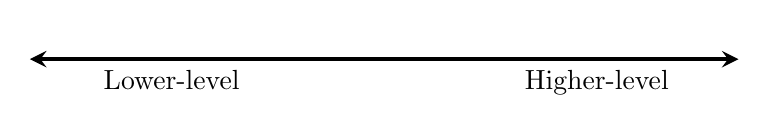
\begin{tikzpicture}
\fill[controlpt] (0,0) circle (0.1);
\draw[arrow] (0,0) -- node[below,pos=0.6] {Lower-level} (-4.5,0);
\draw[arrow] (0,0) -- node[below,pos=0.6] {Higher-level} (4.5,0);
\fill[controlpt] (0,0.3) circle (0.1);
\end{tikzpicture}
\end{center}
\pause
\emph{lightsd opens-up to a wide range of topics.}
\end{frame}

\begin{frame}{Notes on the LIFX bulbs}
\begin{itemize}
\item Get them on sale;
\item Best brightness/colors (AFAIK);
\item Standby power consumption;
\item Cool LAN API, hope they keep it;
\item Only Gen 1 (EOLed in 2015) doesn't crash for me;
\pause
\item \large{\emph{Binary blobs suck.}}
\end{itemize}
\end{frame}

\subsection{Next}

\begin{frame}{``My Roadmap''}
Things I wanna do:
\vspace{1em}
\begin{itemize}
\item Time based releases;
\item Better CI/automation;
\item ``State-enforcement'';
\item Effects API and effects plugins.
\end{itemize}
\end{frame}

\begin{frame}{Not on my roadmap}
Things I wanna have:
\vspace{1em}
\begin{itemize}
\item JSON-RPC extensions: streaming, auth, server notifs;
\item A reversed-engineered LIFX firmware;
\item A firmware that doesn't crash;
\item Support for other brands (Hue?);
\item Color calibration;
\item LIFX stripe support.
\end{itemize}
\end{frame}

\section{Thanks}

{\setbeamertemplate{headline}{}
\begin{frame}
\begin{center}\Huge{Thanks}\end{center}
\vspace{1em}
\begin{center}\Large{\emph{Time for Q\&A and discussion}}\end{center}
\vspace{1em}
\begin{itemize}
\item \Large{\href{https://twitter.com/1opter}{@1opter}}
\item \Large{\emph{\#lightsd} on IRC (\emph{chat.freenode.net})}
\item \Large{\url{https://www.lightsd.io/}}
\end{itemize}
\end{frame}}

\section{Extras}

\begin{frame}{Links}
\begin{description}[pymonome]
\item[LIFX] \href{https://www.lifx.com/}{website}, \href{https://community.lifx.com/}{forum}, \href{https://github.com/lifx}{github}; 
\item[lightsd] \href{https://docs.lightsd.io/current/}{docs}, \href{https://github.com/lopter/lightsd/}{sources}, \href{https://downloads.lightsd.io/}{downloads};
\item[monolight] \href{https://github.com/lopter/lightsd/tree/master/apps/monolight}{sources};
\item[monome] \href{http://www.monome.org/}{website}, \href{http://llllllll.co/}{forum}, \href{https://github.com/monome}{github};
\item[pymonome] \href{https://github.com/artfwo/pymonome}{sources}.
\end{description}
\end{frame}

\begin{frame}{Questions for you!}
\begin{itemize}
\item Hardware hacks?
\item UX with other projects and products?
\item ``Education'' opportunities opinions?
\end{itemize}
\end{frame}

\begin{frame}{Detailed architecture}
\begin{center}
\begin{tikzpicture}
\pic (0, 0) {monolightarch};
\end{tikzpicture}
\end{center}
\end{frame}

\begin{frame}{LIFX products tables}
\begin{tabular}{lll}
\textbf{Generation} & \textbf{Models} & \textbf{Available} \\
\hline
Gen 1 & Original 1000, Color 650 & No \\
\hline
Gen 2 & Color 1000, White 800 & Yes \\
\hline
Gen 3 & A19, BR30, Z (stripe) & Yes \\
\end{tabular}
\par\vspace{2em}
\begin{tabular}{ll}
\textbf{Generation} & \textbf{Notes} \\
\hline
Gen 1 & Has 802.11 and (unused) 802.15.4 \\
\hline
Gen 2 & QCA 4002, AllJoyn, \emph{crashes} \\
\hline
Gen 3 & + versions have IR, \emph{still crashes} \\
\end{tabular}
\end{frame}

\end{document}
